% figures
%h (here) - same location
%t (top) - top of page
%b (bottom) - bottom of page
%p (page) - on an extra page
%! (override) - will force the specified location


\chapter{State of the art}
\label{chap:state-of-the-art}

\section{Chatbots}
From a user point of view, chatbots are trendy nowadays, big companies such as \textit{Google} or \textit{Apple} are pushing to make the technology mainstream. Even if not every lambda people understand the word Chatbot, they all have at least a mental representation of it. Indeed, they could call it Digital Assistant, Siri, Ok Google, etc, in the end they all understood the concept of an artificial intelligence narrowed to more or less human-like conversations.

\subsection{History of Chatbots}
When are they coming from? Not mentioning \textit{Alan Turing} or \textit{Joseph Weizenbaum}, who are considered as the fathers of \gls{ai} and chatbots, would not be fair. Indeed, they forecasted in 1950, that computers will be able to use human-like communication and they proposed a test to distinguish humans from machines, called the Turing Test. Where a human is asked to talk to a masked entity, and determine if it is talking to a human or a computer. If the human cannot determine who is the computer, then the machine passed the Turing test, as seen on figure ~\ref{fig:wikipedia_turing_test_img}. 

In 1966, Joseph Weizenbaum wrote Eliza, a computer program simulating a psychotherapist, which could be seen as one of the first well known attempt to make a chatbot passing Turing test. Note that due to technical restrictions, Eliza is not performing well at all time. As it is for today, it is possible to play with it at on a dedicated website. \cite{chatbot:eliza}

Since Eliza, a lot of progress has been made, indeed, to only cite a few noticeable chatbots: \textit{Parry} (1972), \textit{Jabberwacky} (1988), \textit{Dr. Sbaitso} (1992), \textit{A.L.I.C.E} (1995), \textit{Smarterchild} (2001), \textit{Watson} (2006), \textit{Siri} (2010), \textit{OK Google} (2012), \textit{Alexa} (2015), \textit{Cortana} (2015), Facebook Bots (2016), and \textit{Tay} (2016), which where all part of the Chatbot history \cite{chatbot:futurism_history_infography}.

From IF-ELSE, \gls{aiml}, up to \gls{ml} with \gls{ann} and \gls{dnn}, the improvement in the field of chatbots increased drastically over the years. At every iterations, the algorithms where becoming more sophisticated and better at using the human language, which are now called the field of the \gls{nlp} and \gls{nlu}.

\begin{figure}[h]
    \centering
    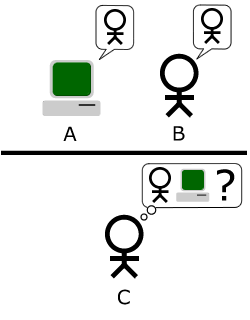
\includegraphics[width=\textwidth,height=6cm,keepaspectratio=true]{Turing_Test_version_3}
    \caption{
       The "standard interpretation" of the Turing Test, in which player C, the interrogator, is tasked with trying to determine which player - A or B - is a computer and which is a human. The interrogator is limited to only using the responses to written questions in order to make the determination. \cite{wikipedia:turing_test_img}
    }
    \label{fig:wikipedia_turing_test_img}
\end{figure}



\subsection{Narrow}
Once again, chatbots are almost everywhere nowadays. Indeed, it became a commun tool for companies of any size to communicate with their customers and a toy for users. However, most of the time, Chatbots are not understood by their users, and is leading to a high level of frustration. Even if they are becoming increasingly mainstream and sophistical, people doesn't realise their limits. Today's chatbots are often mistaken for \gls{agi} as it's seen in \gls{scifi} and are expected to do much more than they are able to do. Indeed, we are making \gls{ani} Chatbots, which implies a specialisation into a specific field.

We should not forget the main purpose of Chatbots, which to provide a conversational service to the user. However, its purpose can be applied in an almost unlimited amount of solutions. Health, Weather, Customer Service, Games, etc. And it could be declined in a text or vocal format.


\subsubsection{\gls{faq}}
With the goal to answer specific questions, \gls{faq} chatbots are probably the most commun type of chatbots. Indeed, their communicational capacities are limited to pre-made sentence and a question answer database, which often results into in the best case scenario a perfect match, or in the worst case scenario something totally unexpected.


\subsubsection{Sequential}
Based on
\subsubsection{Forwarder}
Customer service
\subsubsection{Learning}
\subsubsection{Examples}


\subsection{General}
\subsection{\gls{aiml}}
\subsection{\gls{ir}}
\subsection{\gls{dnn}}
\subsection{Proactive}

\section{Word2Vec}
\subsection{What is Word2Vec}
\subsection{Gensim}
\subsection{Framworks}


\section{Word Embedding Alternatives}
\subsection{FastText}
\subsection{Glove}
\subsection{Word2Vec-f}
\subsection{Wang2vec}


\section{Sentence/Document Embedding Alternatives}
\subsection{Doc2vec}
\subsection{Skip-thought}
\subsection{Smooth Inverse Frequency}
\subsection{RNN}


\section{Datasets}